% Chapter: contains the system architecture

%For every one: use as many diagrams as possible :) (author Petr)

The architecture of \textan{} is based on client-server model. Two main components
are the \textan{} server and \textan{} client which communicate via W3C web services
(SOAP protokol).



\comment{Ondrej}{Mention why it was split like this - a wish from outside, but in 
the future fully automated (tuned) annotation without client}

\comment{Petr}{This explanation should be rather in \ref{sec:Decisions}}

\section{Server architecture}

The server architecture is based on a logical multilayered architecture. It
consists of 5 layers: a presentation layer, a service layer, a business logic layer, 
a persistence layer and a data layer.

\comment{Ondrej}{it definitely needs a figure here, but no generalized pictures, 
it needs your concrete components and connection. The 5 layers sound like textbook example}

\comment{Adam}{The comment above was created when there were no pictures nor subsections 
here, but I have added it anyway, just to be sure}

\begin{figure}[!htb]
        \centering
        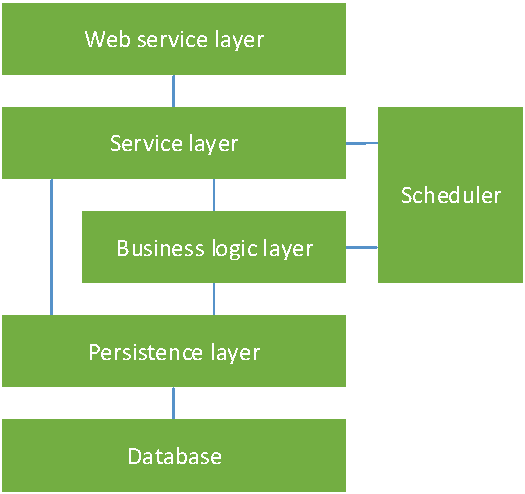
\includegraphics{Images/ServerComponentOverview}
        \caption{Overview of the server layered architecture.}
        \label{fig:ServerComponentOverview}
\end{figure}

\subsection{Web service layer}
Web service layer is the component responsible for providing web service
API. It consists of a servlet container and implementations of particular
web services.

Jetty is used as the servlet container component. It is a powerful and scalable
component which supports embedding into other applications. It also can be run independently
on the rest of the applications. This is an important feature, which allows, that only
web service implementations live in a web context. % I don't understand
In other words, there can be
other implementations over the rest of the application at same time, e.g. from input
command line. This component also provides security of \textan{} server over SSL.

Web service itself is implemented with Apache CXF framework. A bigger part of
the implementation is generated from WSDL files and XML Schema files using the
CXF wsdl2java tool at build time, these classes are placed in the package % which classes?
\emph{cz.\-cuni.\-mff.\-ufal.\-textan.\-commons.\-ws}, the package
\emph{cz.\-cuni.\-mff.\-ufal.\-textan.\-commons.\-models} and its subpackages. % too long and a bit vague
The *.ws package contains java equivalents of a WSDL interfaces and the *.models
package contains java equivalents of XSD complex types. These interfaces are
implemented in classes placed the package \emph{cz.\-cuni.\-mff.\-ufal.\-textan.\-server.\-ws}
and they are just adapters for the service layer. Note that underlaying layers are
totally independent from the web service layer. The CXF framework ensures that
these classes are deployed as servlets.

\subsection{Service layer}
The service layer is a component that consists of classes which handle requests
using underlying layers and register commands in the scheduler. These classes are
placed in the package \emph{cz.\-cuni.\-mff.\-ufal.\-textan.\-server.\-services}
and the package \emph{cz.\-cuni.\-mff.\-ufal.\-textan.\-server.\-models}.

\comment[Petr]{Petr}{Describe all services}

\subsection{Business layer}
The business layer contains components which encapsulate the main functionality
of the system. The layer consists of two main components, the Named Entity
recognizer and the Object assigner. Both of them use machine learning methods to solve
their tasks. They access the persistence layer to obtain training data. They
are called from the service layer and the scheduler.

\subsubsection{Named entity recognizer architecture}

The architecture of Named entity recognizer is divided to two parts: recognition and training.

\paragraph{Recognition} 
Recognition is slitted to two parts - Java part and C++ part. This is because
NameTag, which is the available tool for named entity recognizer, is written mainly in C++. 
TextAn is developed in Java, so we must use JNI to call functions from C++ through provided
Java bindings. C++ part is represented by NameTag, so it has its own documentation.
Java part contains JNI bindings to call C++ part and than connection to TextAn.
This part serves as an adaptor between these two projects. Its main task is
to translate recognized NameTag entities to entities stored in TextAn database.
Because of optimization, this component caches database entities.

\paragraph{Training}
Despite the fact that NameTag is in C++ and TextAn in Java, it is not requisite 
to implement JNI, because training is called as binary files and the model is generated
as file. Therefore, calling C++ functions is not needed. Java part provides
training data collecting from database and preparation, model handling
(deleting old ones. binding them to NameTag).
\comment[Jakub, Petr]{Tam}{Approved?}

\subsubsection{Object assigner architecture}

\comment[Tam]{Petr}{here should be description of TextPro}

After calling \emph{Named entity recognizer}, a list of entities is extracted from the document. \emph{TextPro}
package \emph{cz.cuni.mff.ufal.textan.textpro} automatically
assigns those entities to available objects in database. As the output, for 
each entity, the aforementioned package returns a list of potential objects along
with their score. Two methods are provided.

\paragraph{HeuristicRank}
The most simplest solution is searching for the \textit{objects} with matching 
\textit{alias}. However, for an array of entity, it would return an array of 
list of unordered objects.
Function \emph{cz.cuni.mff.ufal.textan.textpro.HeuristicRanking} loops through 
the whole structure, promote the pair of objects which has a relation. This is 
due to the fact that such pair of objects is more likely to appear in the same
document. However, as a heuristic method, its main role is to guarantee a decent
output for every input.

\comment{Tam}{TODO: Picture for heuristic ranking}

\paragraph{MachineLearning}
Without extensive human effort, machine learning is the best method to achieve
high performance from a huge database. The problem of ``matching potential objects
to an entity'' is reformulated to fit the definition of a classification machine 
learning. Each object is paired with the entity. Then the pair is classified as
\emph{positive} if the object is potentially matched the entity. On the contrary,
the pair is classified as \emph{negative}. It becomes the problem of binary 
classification.

\paragraph{Learning}
The package \emph{cz.cuni.mff.ufal.textan.textpro.data} supports all steps for machine
learning including training (learning). The database is extracted. 
\emph{cz.cuni.mff.ufal.textan.textpro.data} creates 
artificial pairs of training vectors with \textit{Weka} tool. When a new document is
processed, new entity and object pairs is added to the database. They could be extracted
later to train again.

\paragraph{Assigning}
To assign the entity to object, function \emph{distributionForInstance} to return the 
probability of the pair with regards to \emph{positive} class. The probability value 
is ranked an used as the score.

\comment{Tam}{TODO: Features description, maybe}
\comment[Tam]{Adam}{Yes, the more the better ;-)}

\paragraph{Features}

The feature set is selected among evaluations with regards to the pair between
the entity and the object. A feature could be computed by comparing the entity 
and the object. It also may be the characteristics of the entity or the object 
alone. All the selected features are considered to form a meaningful set which
expresses the nature of the pair. In the Assigner, the feature set is selected 
as follow:

\begin{itemize}
\item The String distance metrics between the entity text and the object aliases. Given 
the fact that an object may have more than one alias, the package computes three numbers for 
\textit{similarity} between the entity text and the object aliases: the highest, the lowest and
the average. It is to distinguish between an object with one alias and object with hundred aliases.
\item The type comparison between object type and entity type. If a pair is \textit{positive},
the types have to be the same. This is a crucial features. 
\item The number of aliases that the object has.
\item The number of documents that the object appears.  
\end{itemize}


\subsection{Scheduler}
The scheduler is a simple component, that invokes commands asynchronously against
requests in the servlet container. It is implemented by classes in the package
\emph{cz.\-cuni.\-mff.\-ufal.\-textan.\-server.\-commands}.

\begin{figure}[!htb]
        \centering
        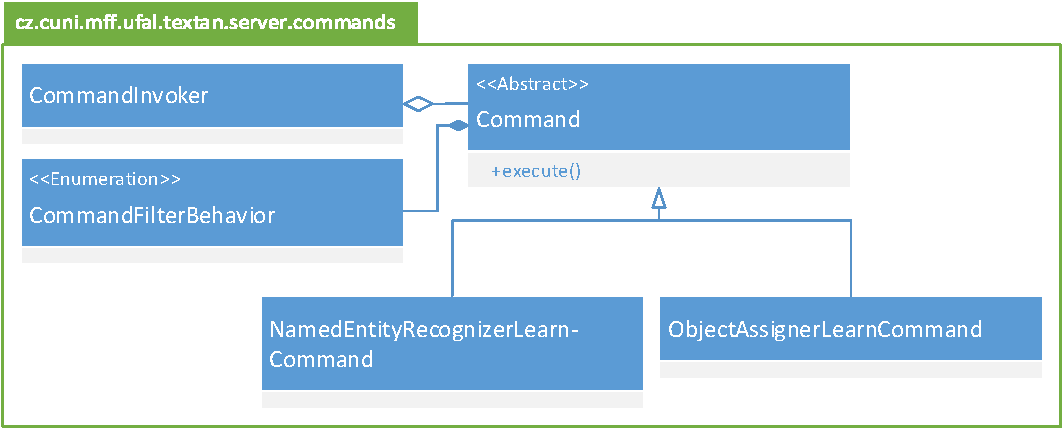
\includegraphics[width=\textwidth]{Images/Commands}
        \caption{Overview of the scheduler classes.}
        \label{fig:CommandsOverview}
\end{figure}

The component is used to invoke re-learning in components from the business layer.
The learning is typically slow, in a matter of minutes, so it's necessary to use
this approach due to system performance. Commands are registered from methods in
the service layer that modify data used for learning. Commands are stored in one
FIFO queue and are invoked in one thread, so it's possible to filter them before
invocation. This ability ensures that only one learning command is invoked at one
time and that learning commands are not invoked unreasonably. Components from
the business layer use old models during learning, so the re-learning is a transparent
operation for users.

\subsection{Persistence layer}

\comment[Venca]{Petr}{Describe DAOs, database mapping, underlying database etc.}

\comment[Petr]{Petr}{Describe full text indexing: hibernate search, lucene, a their mappings}

\comment[Petr]{Petr}{Describe new Czech analyzer}

Persistence layer cares about providing data to application layer and ensure they are persistent.
First of all this layer needs to convert data between database and objects in java. This is called Object-Relation Mapping (ORM). Java classes whose instances are stored in database tables are called persistent classes. And we need to persist these objects. That is where Hibernate comes to the scene (see section \ref{ssec:UsedLibraries}) and do that for us.
Next thing we need take care of is to perform a transaction, for example joining two objects should first check if they are roots and if so, they are joined. All operations with database are usually done by DAOs.
\begin{figure}[!htb]
        \centering
        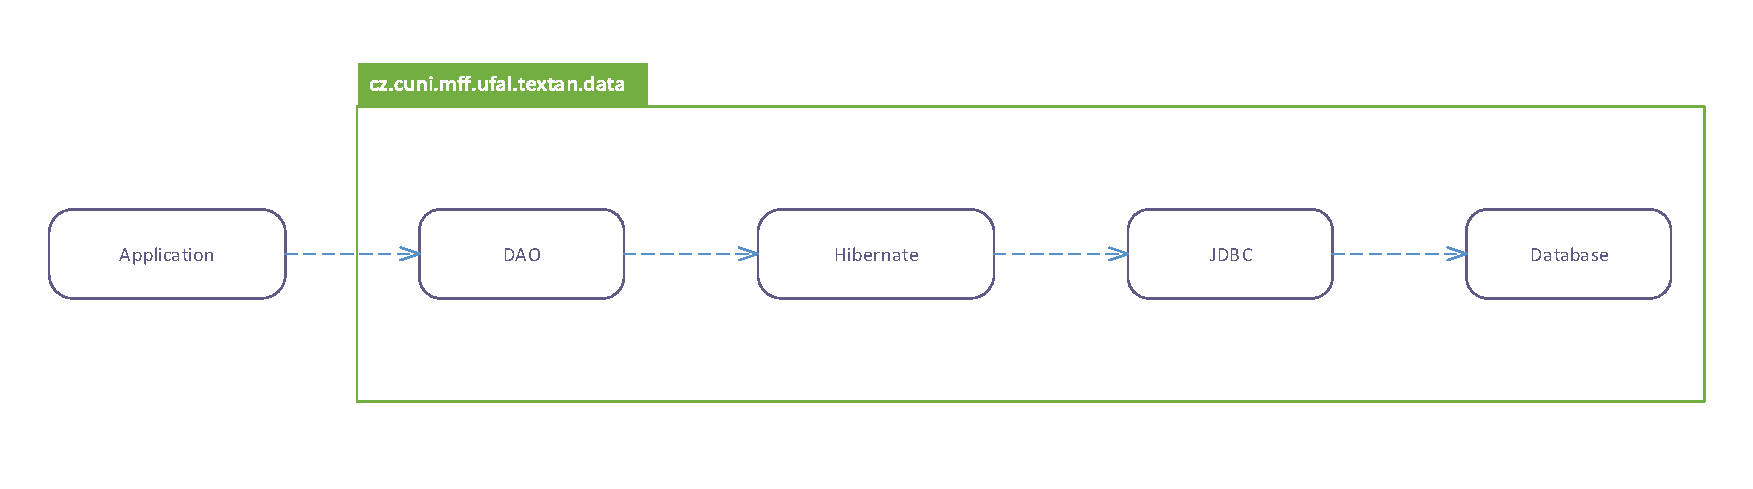
\includegraphics[width=\textwidth]{Images/PersistentLayer}
        \caption{Persistence Layer}
        \label{fig:PersistentLayer}
\end{figure}
Data Access Object (DAO) is a basic design pattern for most of enterprise applications and wraps all access to data sources. It also handles the connection to data sources to get and store data. What is good for? Basically it's appreciated when the persistence layer changes. For example if we decide not to use hibernate but some other library, we don't have to remake the whole application but only the DAO and all under it.
As you can see in figure \ref{fig:PersistentLayer} without DAO would have the application to call Hibernate functions and it would be dependent on Hibernate. Now the application don't know anything about hibernate and if we are using it or any other ORM.

\begin{figure}[!htb]
        \centering
        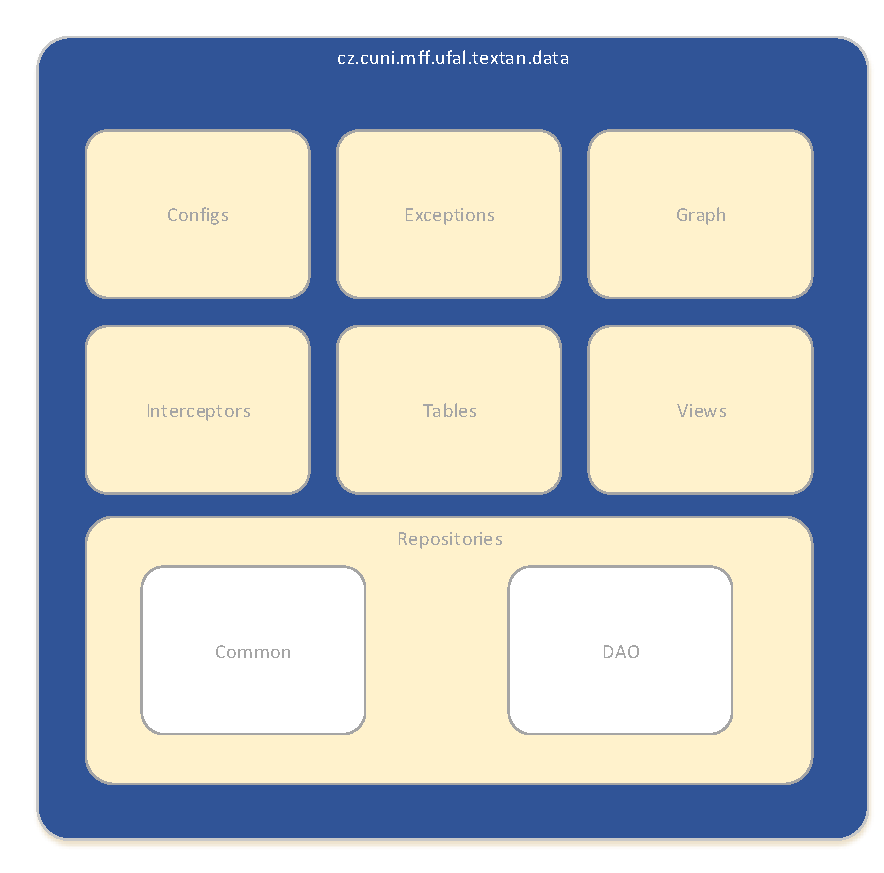
\includegraphics[width=\textwidth]{Images/DataDecomposition}
        \caption{Persistence Layer Decomposition}
        \label{fig:DataDecomposition}
\end{figure}



As you can see in figure \ref{fig:DataDecomposition}, our persistence layer is covered by package \emph{cz.cuni.mff.ufal.textan.data}. In this section when we mention some subpackage, we always mean the subpackage of the package \emph{data}.

The mapping between tables in database and java classes is done in subpackage \emph{tables}. Every table in database corresponds to a class that extends \emph{AbstractTable}. Hibernate did the mapping for us. 

\begin{figure}[!htb]
        \centering
        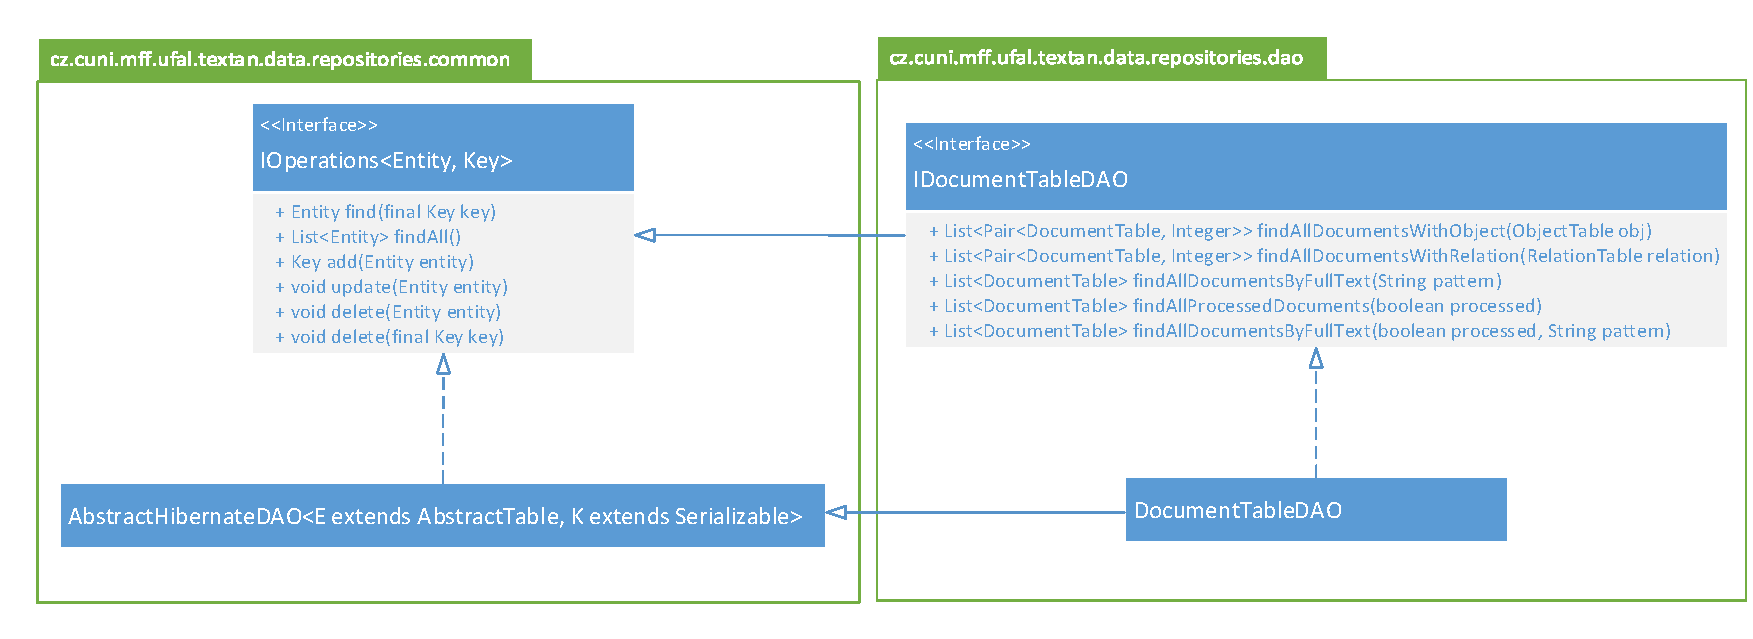
\includegraphics[width=\textwidth]{Images/DatabaseDAO}
        \caption{DAO Example for Document Table}
        \label{fig:DatabaseDAO}
\end{figure}

To provide the data to application (server in our case) we have used the DAO pattern as we mentioned earlier. DAOs are located in subpackage \emph{repositories}. On figure \ref{fig:DatabaseDAO} is an example of a DAO pattern for document table. Interface \emph{IOperations} describe common methods for all tables and AbstractHibernateDAO implements them. Now we have for example the document table, we have interface \emph{IDocumentTableDAO} that describes all operations with document table and \emph{DocumentTableDAO} implements them for Hibernate. The application (server) itself shouldn't know about the implementations to guarantee the independence on Hibernate.

Another subpackage \emph{graph} contains all necessary methods to generate a graph from database. Nodes of this graph represents objects and relations in database. Edge between an object and a relation means that this object is in that relation. We have used the factory pattern to create graph. There are methods in class \emph{GraphFactory} to generate a graph from an object to given depth and also supports finding shortest path between two objects. For this has been used the Floyd-Warshall algorithm. 

%TODO finish shit about floyd warshall implementation
\comment{Venca}{Finish shit about floyd warshall after implementation and problem with memory}

Last interesting subpackage is \emph{interceptors} where are located definitions of Hibernate interceptors. Interceptor is something like trigger in a database. When there is called insert, update or delete action in hibernate, a propper method in an interceptor is called. We are using it for \emph{global version} which we discuss in next section \ref{sec:Database}.


\subsection{Database}
\label{sec:Database}

\comment[Venca]{Petr}{Describe database: database schema etc.}
This section describes the database schema (see figure \ref{fig:DatabaseSchema}), meaning of all database tables and columns.


\begin{figure}[!htb]
        \centering
        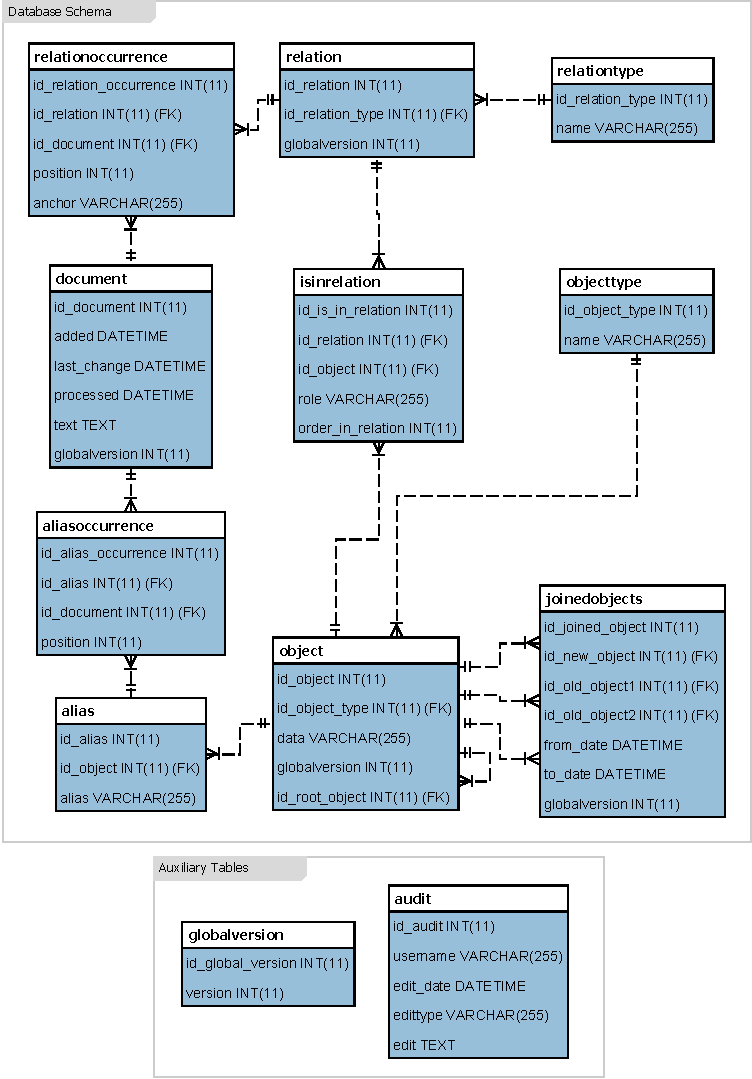
\includegraphics[width=\textwidth]{Images/DatabaseSchema}
        \caption{Database schema}
        \label{fig:DatabaseSchema}
\end{figure}

\paragraph{Document} The report to be processed. In the database, there are columns for the date of 
creation \emph{(added)}, the date for last change and the date when the document has been processed.

\paragraph{Object} Object stands for the entity e.g. Josef Novák or a specific address. 
The table has only one column with content \emph{data} which is used to describe the object. 
Apart from that, it contains reference to \emph{ObjectType} table to determine what type the object is.

\paragraph{Object Type} The \emph{objecttype} table is used to describe if an object is a human or an address. 
It has only one column with name of the type and the type have to be unique.

\paragraph{Alias} If an entity occurs in some document, we want to 
know how did we call them. For instance Josef Omáčka can be called as 'Josef', 
'Pepe' or 'Killer'. Alias table represents all these possibilities (aliases) 
of a specific entity.

\paragraph{Relation} There may be relations between entities, for example killer-victim,
mother-son, live, use, etc. This table describes such relationship. 

\paragraph{IsInRelation} There can be relation among more than two entities, for example 
killer-victim-place-time. This is the reason we have used the N:N relation 
between \emph{object} and \emph{relation} tables, which represents the \emph{isinrelation} 
table. For instance, to distinguish between killer and victim, the column \emph{role} 
(more user friendly) and \emph{order\_{}in\_{}relation} have been used.

\paragraph{RelationType} As well as the objects have types, the relations have their type too. 
For example \emph{kill}, \emph{live} or \emph{sell}.

\paragraph{Relation and Alias Occurrences} These two tables stand for the occurrence of an 
alias and relation in a document respectively. It contains their beginning positions in the document 
and an anchor for relation. 

\paragraph{Joined Objects} It is possible that users may realize two different entities are actually 
a single one. In this case, two objects have to be joined into a new one. This can be done by 
\emph{joinedobjects} table. However, this join can be a wrong decision. There is a column 
to\_{}date in case these merged objects are separated.

\paragraph{Audit} All inserts, deletes and updates in the tables above are being saved into \emph{audit} 
table. It is a simple table because it keeps a string of modified object. It also 
keeps username of the user who performed the operation, the date of the change and what kind 
of change was processed.
 
\paragraph{Global Version} Before finishing the process of a document, it is checked whether there
are other documents which have been added or modified. To perform that check we need to have some information
when the tables have been modified. Tables \emph{Document}, \emph{Object} and \emph{Relation} 
contain a column \emph{globalversion}, which increments with each insert, delete or update. 
Current global version is stored in \emph{globalversion} table where there is only a single row every time.

\paragraph{} As you may see, there is a little bit of redundancy in our schema. There is alias table where the alias of an object is stored. But if we really want to extract the alias of an object, we could get the alias from document, which the object occurs. However, that would be too complicated to get from single query. Furthermore, we want a method to easily get all aliases of an object.
Next redundancy is \emph{Object.id\_{}root\_{}object} which is a foreign key of the same table. Once we join objects and we get a new one, this joining together makes a binary tree. A root of the tree is the object, of which we want to edit aliases, because other objects in the tree are not taken into account. So we need two things: the determine if a given object is a root and the method to get the root if current object is not the root. Without that column we would have to join until we get to the root and that, as we know, can't be done in a single sql query. With the column, we only ask if the root of an object is the same or we simply get the root object in one join.

\section{Client architecture}

\comment[Adam]{Petr}{here should be description of client architecture (MVC etc.)}

\comment{Tam}{NOTE: your sentences are way too long :)}

\textan{} client consist of two main parts. The package
\emph{cz.cuni.mff.ufal.textan.core} and its subpackages handle communication
with webservices and completely hides them from the package
\emph{cz.cuni.mff.ufal.textan.core} and its subpackages which are responsible
for actual displaying the user interface (see figure \ref{fig:ClientOverview}).
It means that the model representation is duplicite to classes generated from
the WSDL by CXF into \emph{cz.\-cuni.\-mff.\-ufal.\-textan.\-commons.\-model}
and \emph{cz.\-cuni.\-mff.\-ufal.\-textan.\-commons.\-ws} and their subpackages.
On the other hand this approach has great advantage - webservice interface
changes will require only code refactoring localized into \emph{core.*}
packages. There is also \emph{cz.\-cuni.\-mff.\-ufal.\-textan.\-tui} package
containing a simple batch report processor without user interaction.

\begin{figure}[!htb]
        \centering
        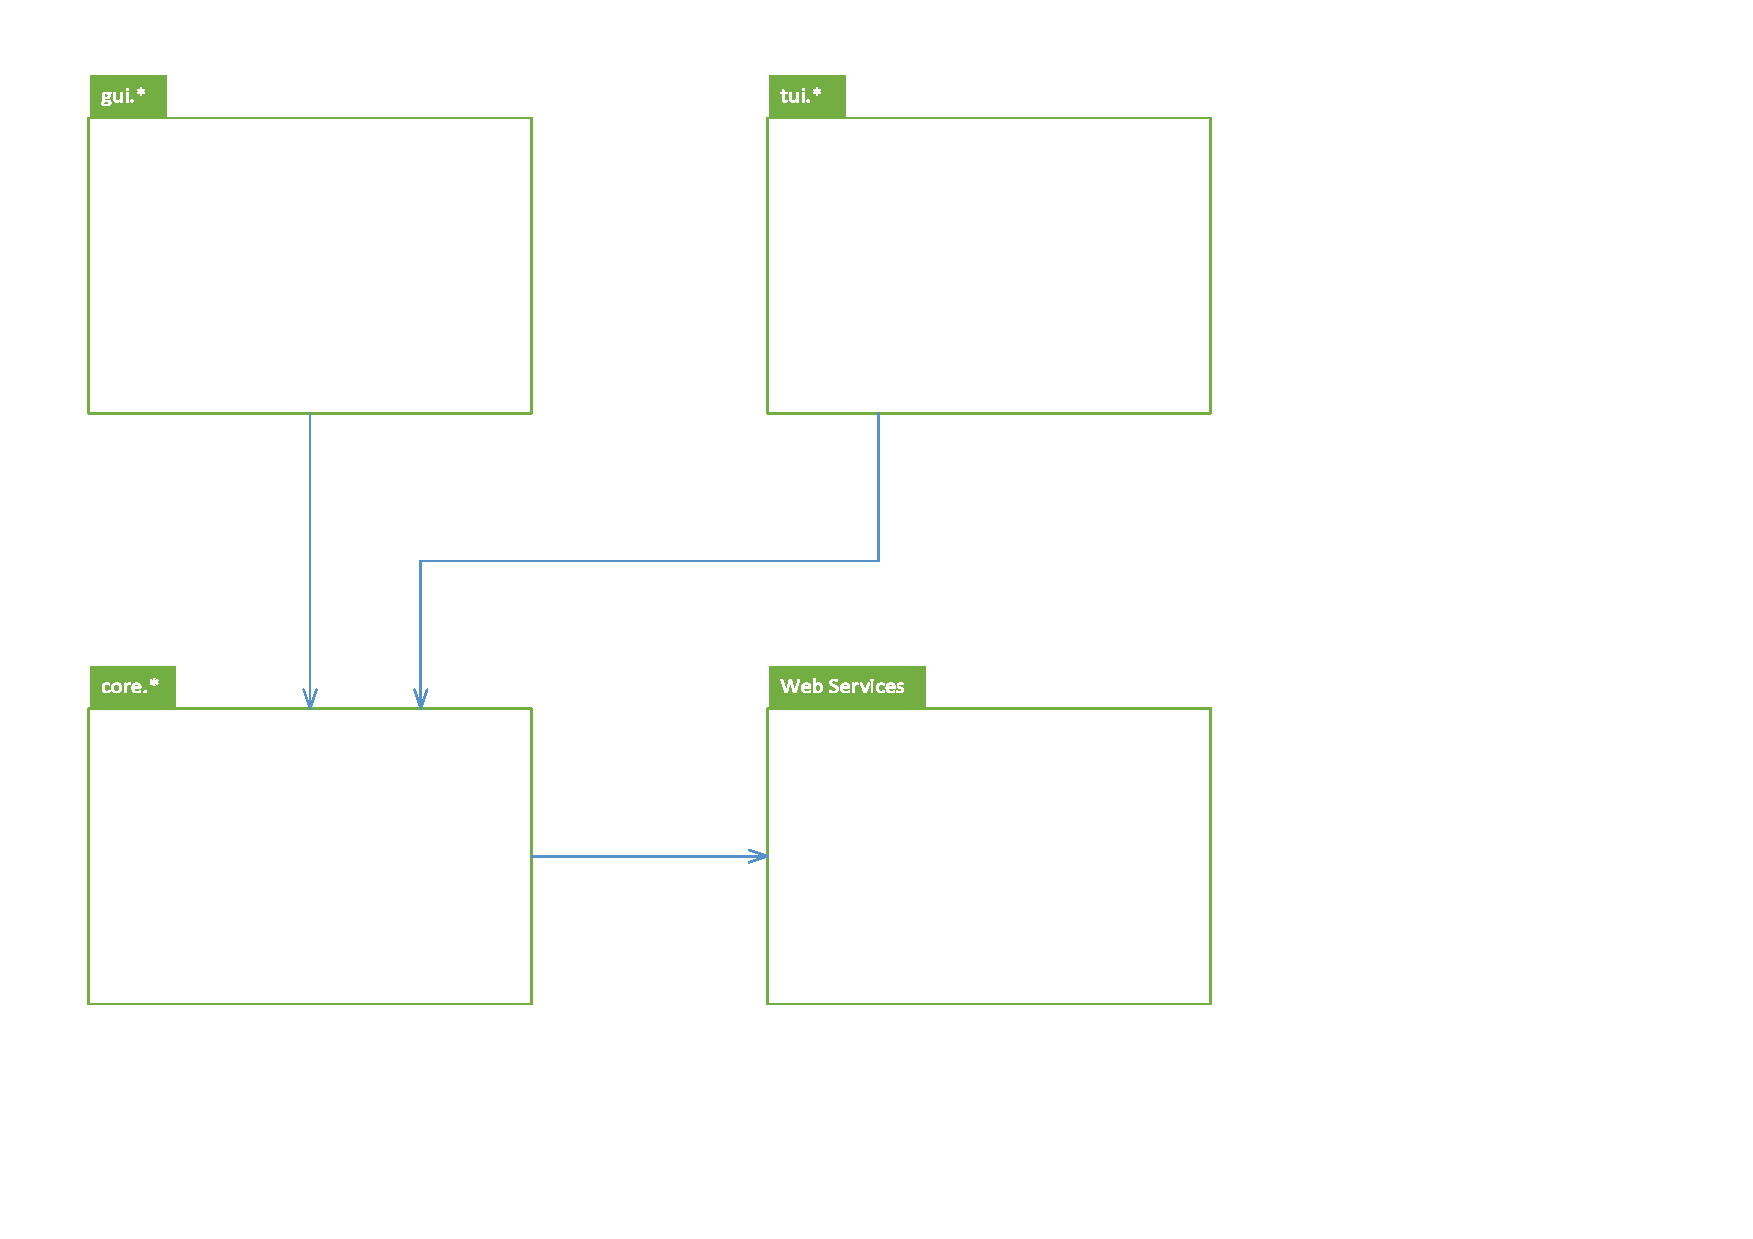
\includegraphics[width=\textwidth]{Images/ClientOverview}
        \caption{Overview of the packages.}
        \label{fig:ClientOverview}
\end{figure}

For visualization itself JavaFX framework is used. It naturally enforces
Model-View-Controller architecture.

In the rest of the section the most important packages will be introduced and
described.

\subsection{Model - cz.cuni.mff.ufal.textan.core}

Model classes can be found in this package. It contains mainly client side
representation of object, entity, relation, document etc. (see figure \ref{fig:CorePackage}). Most important class
is \emph{Client} which is used for communication with the webservices. It also
serves as a factory of \emph{ProcessReportPipeline} (see
\ref{sssec:ReportPipeline}). There are also \emph{SynchronizedDataProvider} and
\emph{SynchronizedDocumentProcessor} to provide synchronization for
\emph{IDataProvider} and \emph{IDocumentProcessor} created by CXF.

Subpackages of the \emph{Core} package focus on individual client side tasks,
like displaying graphs and processing report in a pipeline.

\begin{figure}[!htb]
        \centering
        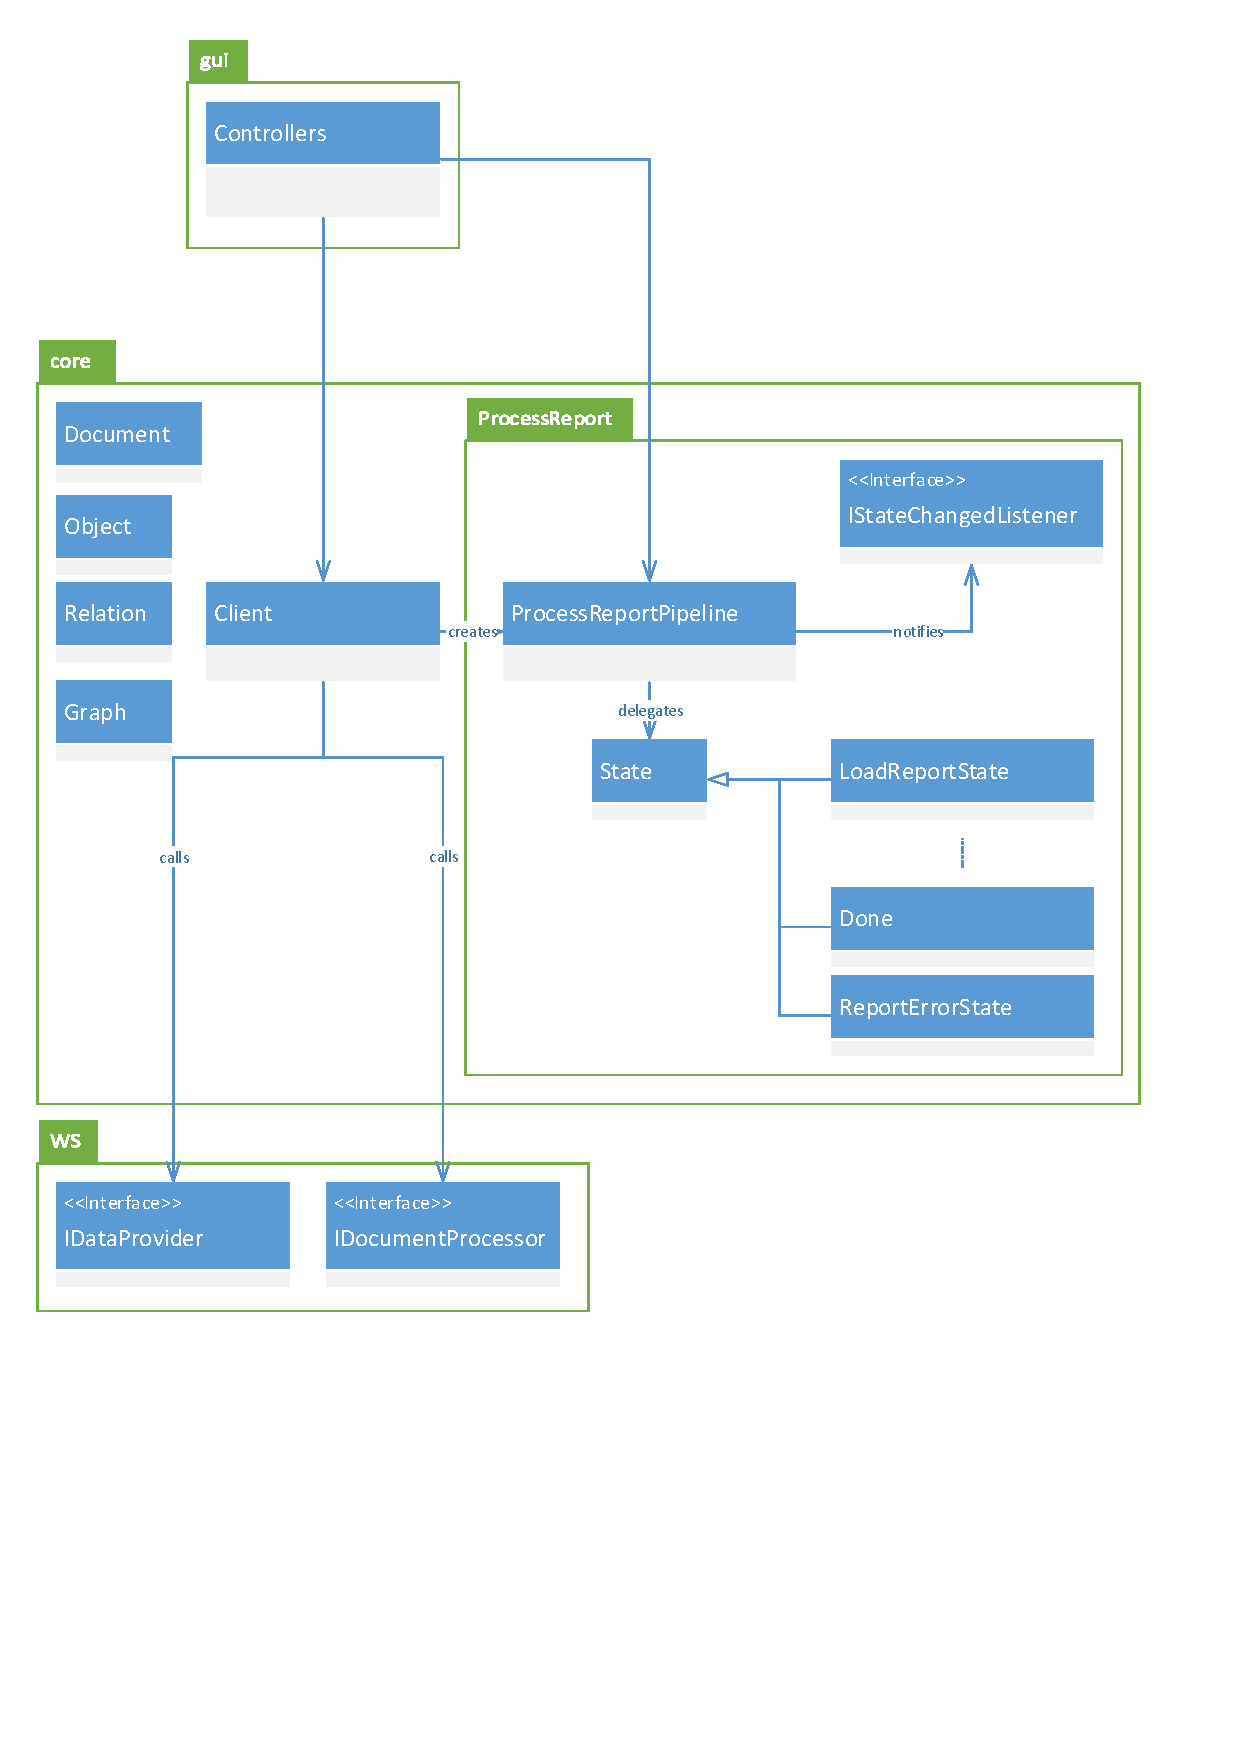
\includegraphics[width=\textwidth]{Images/CorePackage}
        \caption{Overview of the most important features of \emph{core} package.}
        \label{fig:CorePackage}
\end{figure}

\subsubsection{cz.cuni.mff.ufal.textan.core.reportpipeline}
\label{sssec:ReportPipeline}

This package contains classes necessary for report processing (see figure
\ref{fig:CorePackage}). Most importantly there is class
\emph{ProcessReportPipeline} that holds information about processing one report.
The pipeline/wizard approach was chosen because the amount of choices and
required tasks would be overwhelming to users if they were all provided at once.
Virtually all methods of the pipeline object are delegated to its \emph{State}
(see figure \ref{fig:Pipeline}). Descendants of the class \emph{State} are
singletons. They contain most of the pipeline processing logic and control to
which state the pipeline should go next. When this happens, each registered
\emph{IStateChangedListener} is notified.

\begin{figure}[!htb]
        \centering
        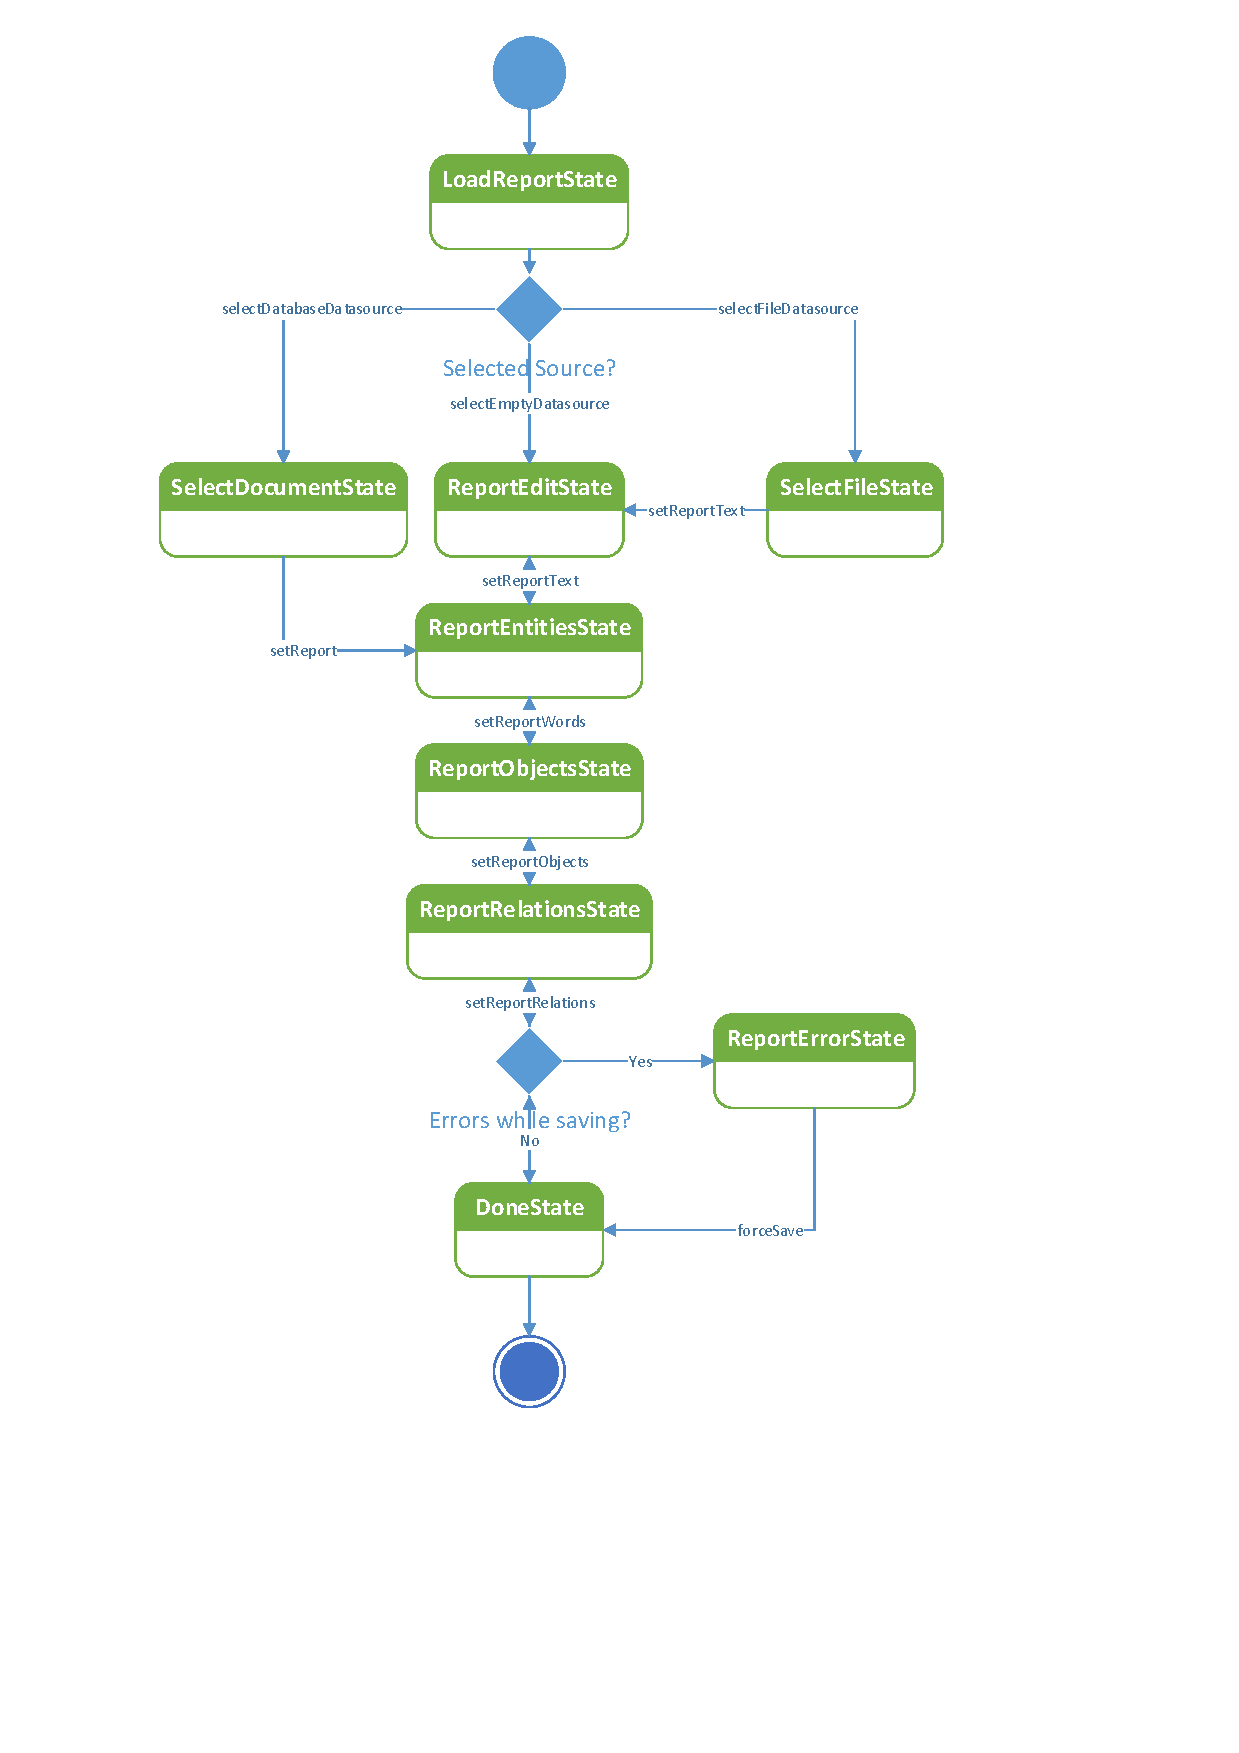
\includegraphics[height=16cm]{Images/Pipeline}
        \caption{Pipeline state machine.}
        \label{fig:Pipeline}
\end{figure}

For easy selecting recognized entities and relations a hierarchy of builders
has been developed (see \ref{fig:Builders}). This is necessary because
\emph{Object} and \emph{Relation} immutable. The \emph{word} is a class
representing independent word of the report text. It can be assigned to either
an entity or relation. \emph{EntityBuilder} also holds the assigned object if
any.

\begin{figure}[!htb]
        \centering
        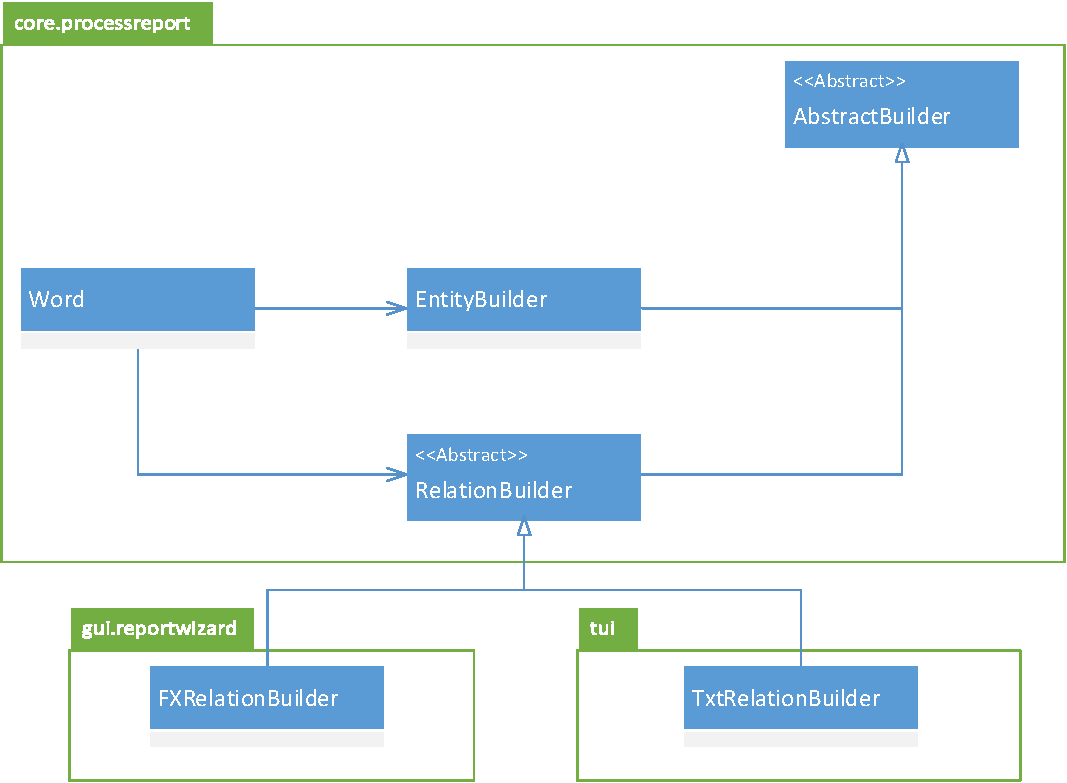
\includegraphics[width=\textwidth]{Images/Builders}
        \caption{Overview of the builders hierarchy.}
        \label{fig:Builders}
\end{figure}

\subsubsection{cz.cuni.mff.ufal.textan.core.reportpipeline.load}

This package contains classes needed for importing report texts from external
files. There is \emph{IImport} interface that provides methods for extracting
text from an array of bytes. Custom implementations of \emph{IImporter} need
to be registered to class \emph{ImportManager} to be selectable by users. The
rest of the package is a few classes providing import of text files in most
common encodings.

\subsubsection{cz.cuni.mff.ufal.textan.core.graph}

This package contains several classes related to creating graphs. They handle
mostly graph filtering which is done solely on client side. See figure
\ref{fig:Graph}.

\begin{figure}[!htb]
        \centering
        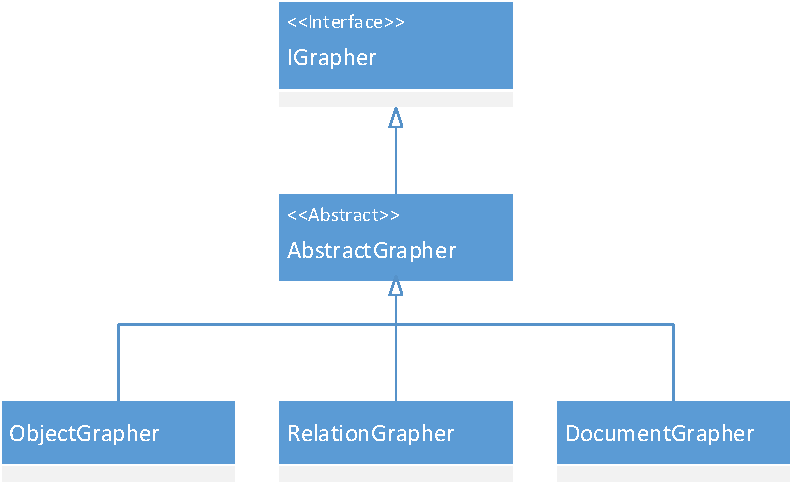
\includegraphics[width=\textwidth]{Images/Graph}
        \caption{Overview of the \emph{graph} package.}
        \label{fig:Graph}
\end{figure}

\subsection{Controller and View - cz.cuni.mff.ufal.textan.gui}

This package and its subpackages contain controller classes and several view
components that had to be customized to achieve specific behavior. A hierarchy
of controllers has been developed, mostly for code reuse (see
\ref{fig:Controllers}). Controllers extensively use \emph{core} package.

\begin{figure}[!htb]
        \centering
        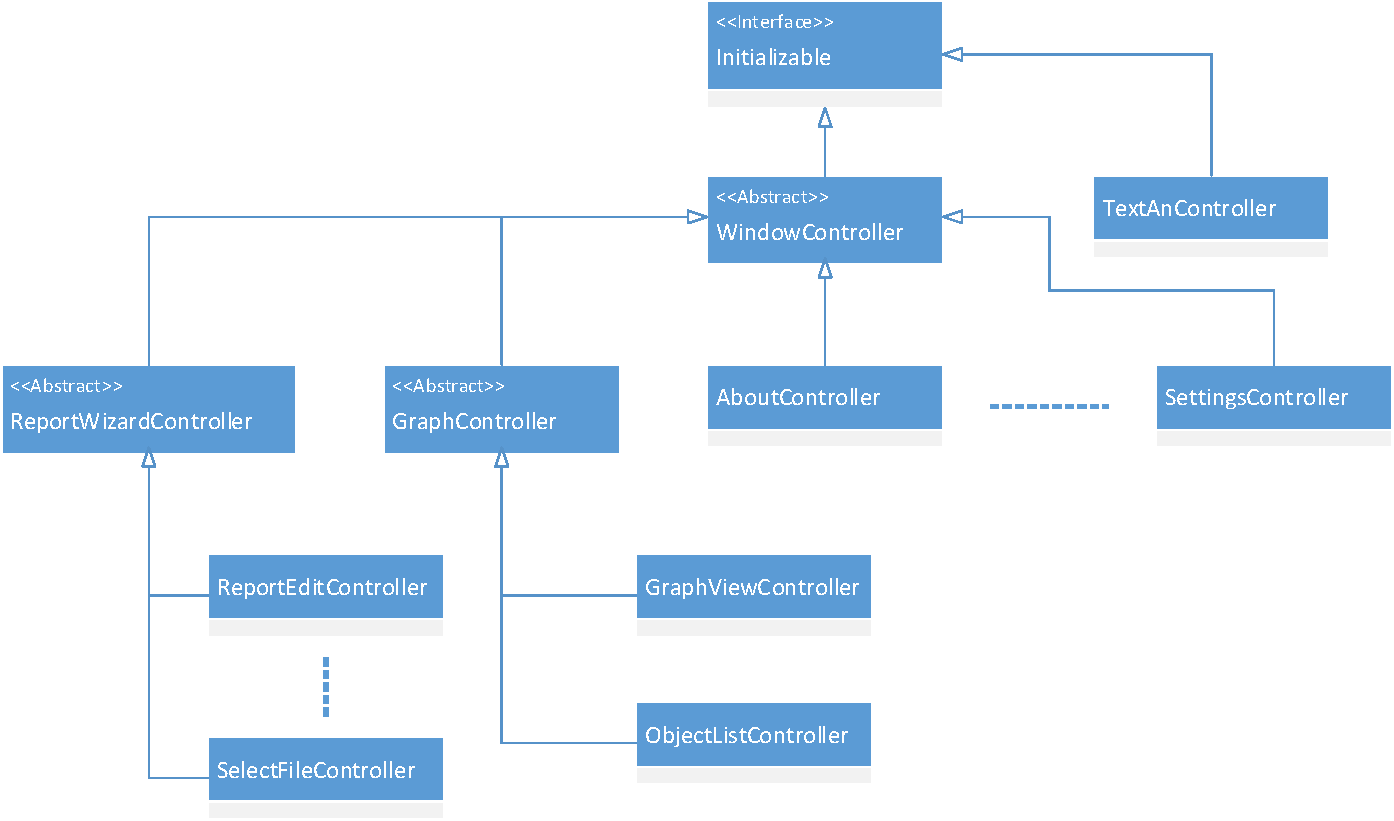
\includegraphics[width=\textwidth]{Images/Controllers}
        \caption{Overview of the controllers hierarchy.}
        \label{fig:Controllers}
\end{figure}

Resources from this package and its subpackages contains descriptions of views
(*.fxml files), styles (*.css files) and localization (*.properties files).

\begin{figure}[!htb]
        \centering
        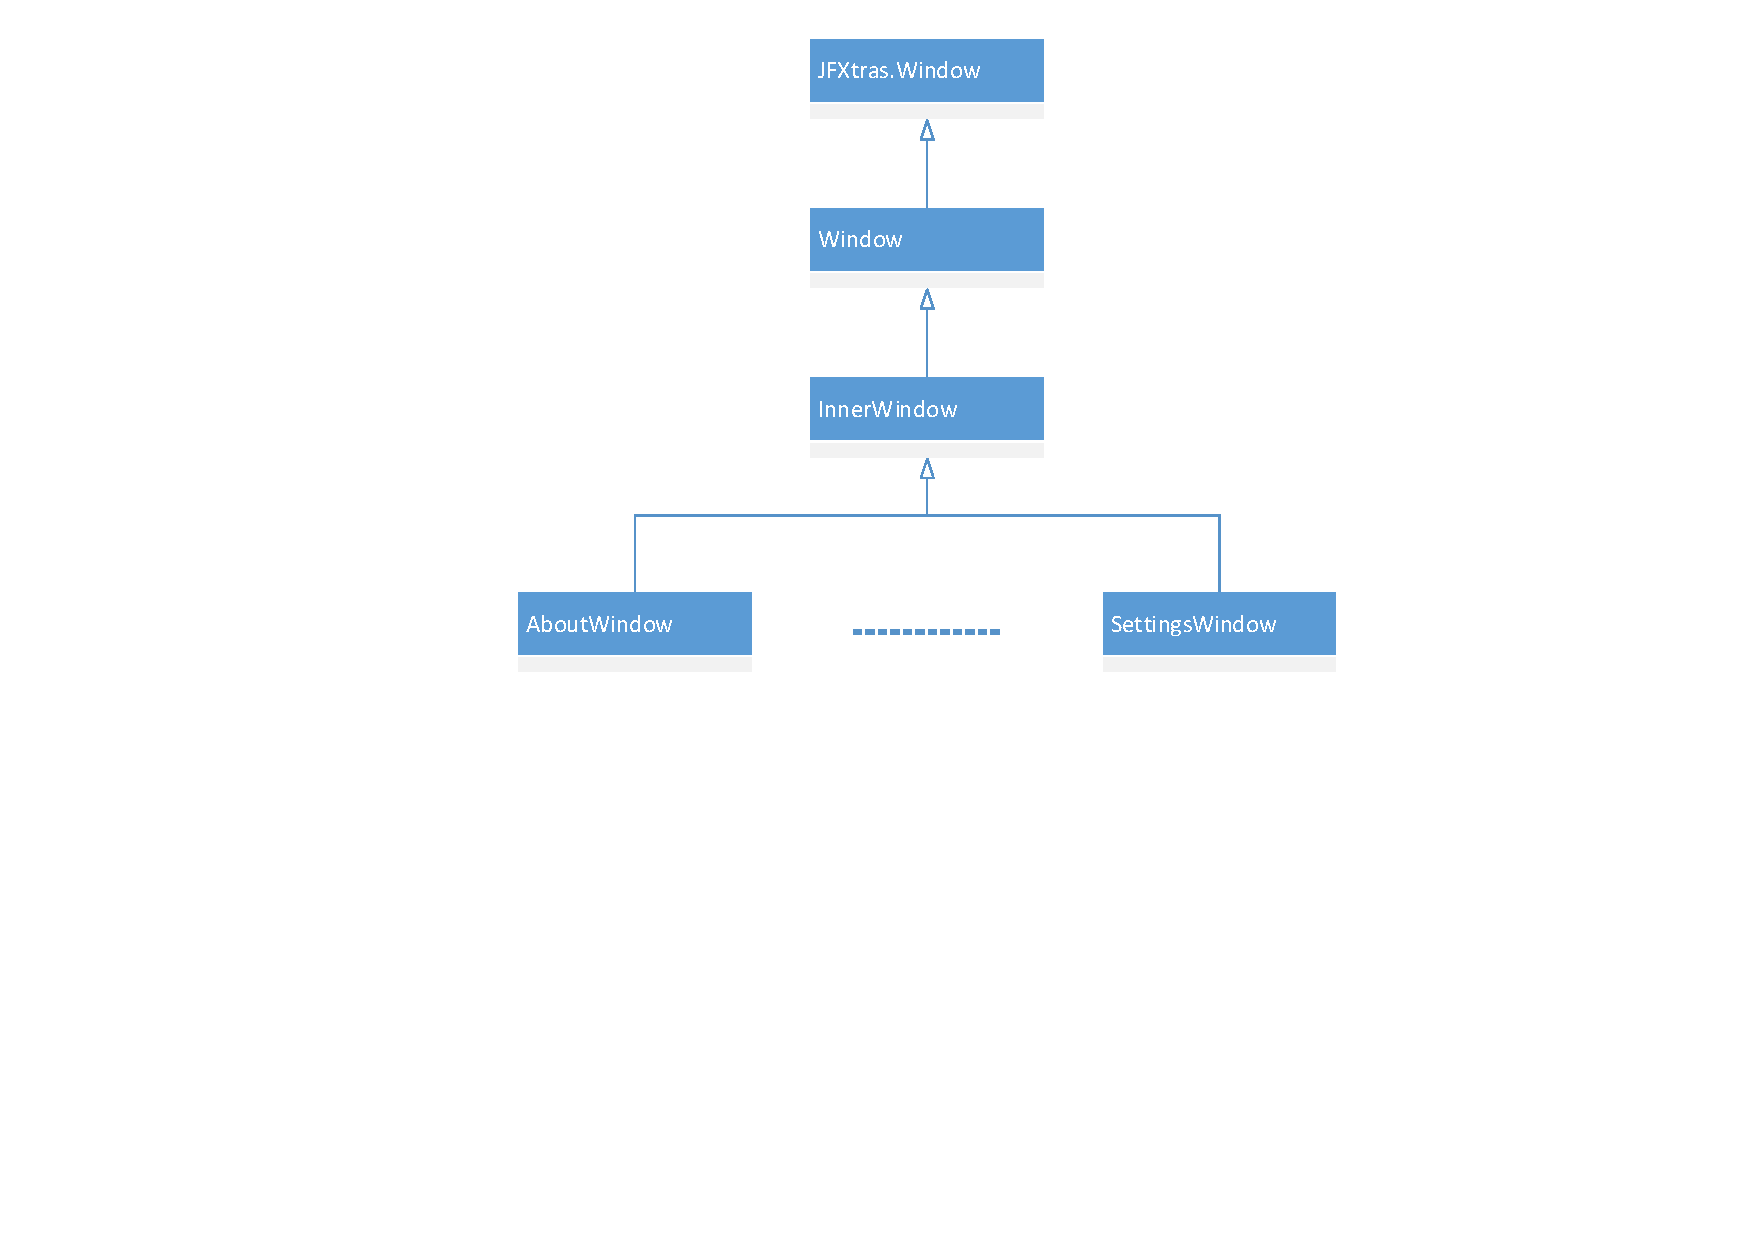
\includegraphics[width=\textwidth]{Images/Windows}
        \caption{Overview of the windows hierarchy.}
        \label{fig:Windows}
\end{figure}

\subsubsection{cz.cuni.mff.ufal.textan.gui.graph}

This package contains controllers for objects and graph views. The most
interesting class is \emph{GraphView} which embeds JUNG Swing graph into JavaFX
and inserts content of \emph{cz.cuni.mff.udal.textan.core.Graph} to JUNG graph.
Also handles hypergraph conversions if needed for which it uses auxiliary
classes \emph{DummyRelation} and \emph{RelationObject}.

Its only subpackage \emph{string} contains only class \emph{Handler}. It is a
workaround that copes with inability of JavaFX to load css style sheets from
\emph{String} which is needed for \emph{GraphViewController} to generate styles
for coloring filter list checkboxes. For that reason custom url schema "string"
has been created and \emph{Handler} resolves it with strings registered to it.

\subsection{Used Libraries}
\label{ssec:UsedLibraries}

\comment[Adam]{Adam}{Find a suitable place for this section and refactor it.}

\paragraph{ControlsFX}
ControlsFX is a Java8 open source library aiming at enhancing the programming
experience with standard JavaFX. It provides wide selection of new and improved
components to make everyday use of JavaFX even easier. \textan{} uses it mainly
for its high quality and user-friendly standard dialogs which are
incomprehensibly and sorely missing in JavaFX.

\paragraph{JCommander}
JCommander is a very small Java framework that makes it trivial to parse command
line parameters. It was chosen because of easy to used annotaion API and no
external dependencies.

\paragraph{JUNG}
JUNG (Java Universal Network/Graph Framework) is older Java library for
displaying graphs, still widely used in Java world, well documented and easily
extensible. Sadly, it does not support JavaFX, but only older Java GUI framework
SWING. Fortunately, thanks to new JavaFX8 SwingNode enabling usage of SWING
components in JavaFX scenes it was possible to seamlessly integrate JUNG into
JavaFX \textan{} Client.

\paragraph{JFXtras}
JFXtras is another JavaFX8 enhancing project. \textan{} Client uses it mostly
for its window management capabilities enabling extensible use of inner windows
embedded into the main window. Another used component is BigDecimalField which
brings common Spinner component into JavaFX.

\comment{Ondrej}{I do not know at all what I should imagine under last sentence.}

\paragraph{PretopoLib\footnote{\url{http://pretopolib.complexica.net/}}}
Although JUNG is mature and well thought library, it lacks one important feature
out-of-the-box: displaying hypergraphs. For this reason JUNG graph rendering
part of PretopoLib is used. PretopoLib is a library mainly focusing on
pretopology and graph displaying is rather byproduct. However it fully meets our
requirements and its author kindly provided us the sources so we could fix one
inconvenient detail.

\section{Communication}
\label{sec:Communication}
\comment[Petr (\& Adam)]{Petr}{Describe communication pattern between client and server,
sequence diagram etc.}

A communication between the client and the server is stateless, because the processing
of a document by a human user may take a very long time, especially because of the saving
of documents during processing in the client. Sessions cannot be used on
the server side, because they can die due to timeout before end of the processing.
For this reason, the state of a processing is placed on client side and is transferred
with each request in situations where it is necessary.

Usage of webservice \emph{DataProvider} is straightforward, its operations are
completely independent and are intended for viewing and manipulating
the database.

The service \emph{DocumentProcessor} is more demanding and needs its operations
called in specific order to achieve proper recognition (see figure
\ref{fig:ClientServerCommunication}). First of all, the client needs to obtain
the ticket which stores information about processing and is needed for all
following calls. For three recognition operations there are two variants. First
for processing report already stored in the database (called\emph{*ById}) and
second for inserting completely new document to the database (called
\emph{*FromString}). Operations \emph{getEntities*} recognize entities in
given report. Operations \emph{getAssignments*} assign objects from the database
to recognized entities and finally operations \emph{getRelations*} recognize
relations between objects. Please note that \emph{getRelations*} is not
implemented in this version of \textan{} and returns empty response with no
relations.

The recognition operations do not store anything into the database. For this
purpose there are three operations \emph{saveProcessedDocumentFromString} and
\emph{saveProcessedDocumentById} with similar differences as mentioned above.
The third operation \emph{rewriteAndSaveProcessedDocumentById} has as input
parameters both document id and document text, because it overwrites the report
text stored in the database. It is intended to be called when the document has
been changed by others while being processed by the user, so the user can
force returning to the original version or provide new one. All three operations
take \emph{force} parameter specifying whether the saving should happen even
though there have been external changes to the database, e.g. new objects, new
relations and newly joined objects.

If the \emph{force} parameter is \emph{false} and such external changes have
been detected, saving returns \emph{false} and method \emph{getProblems} can be
called to get information about the changes. After making adjustments to
recognizing/assignments if needed, save operations can be called with
\emph{force} parameter set to \emph{true}.

During the processing of a document already stored in the database, other users
can alter it in the database. If this happens, the subsequent call of processing
operation returns fault \emph{documentChangedException} as a warning. If the
user wants to overwrite these changes as mentioned above, the client should
switch to \emph{*FromString} recognizing operations and save the report with
operation \emph{rewriteAndSaveProcessedDocumentById}.

If the document stored in the database has been processed by another user while
being processed by a local user, the subsequent call of processing operation
returns fault \emph{documentAlreadyProcessedException} and the processing must
end as no report can be processed multiple times.

For more details, consult the WSDL descriptions and Javadoc of the server
implementation.


\comment{Adam}{It could be interesting if the sequence diagram is extended to include server components too.}
\comment{Petr}{Maybe only for some communication, definitely not all}

\begin{figure}[!htb]
        \centering
        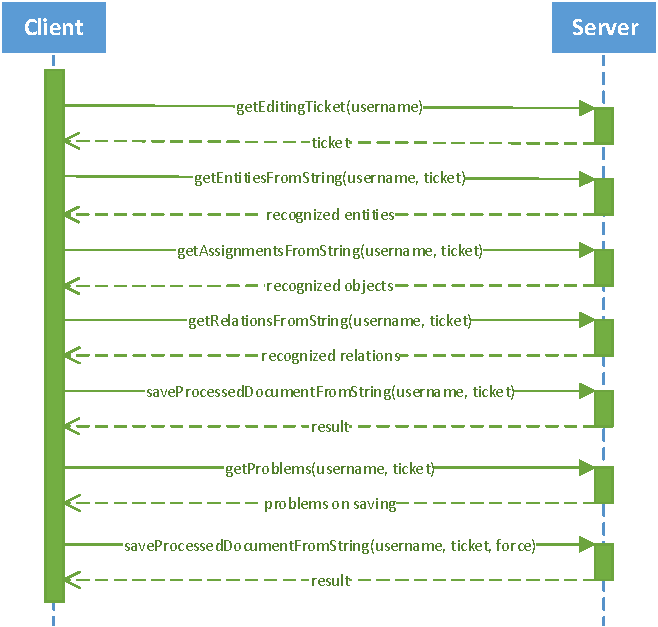
\includegraphics[width=\textwidth]{Images/ClientServerCommunication}
        \caption{Example of Client-Server communication during report processing.}
        \label{fig:ClientServerCommunication}
\end{figure}
